\chapter{Používané metody testování}
V této kapitole se pokusím popsat co nejvíce známích pohledů a způsobů na testování, aby bylo dále možné vybírat, aplikovat a navrhovat testovací systém s ohledem na dnešní metody a trendy v testování. Nejdříve budou popsány úrovně testování, kterými by měl daný výrobek projít, dále popíši způsoby jak testování může probíhat. V poslední kapitole jsou popsány další možné pohledy a přístupy k testování.

\section{Úrovně testování}
Testování výrobků prochází několika stupněmi testování. Některé stupně jsou při vývoji používány bez toho aby jsi to vývojáři uvědomily a některé zase opomíjeny. Mnou rozebíráný model má celkem 5 stupňů testování.  Jednotlivé stupně dále popíši a rozeberu jejich přínos v testovací systému.

\begin{figure}[h]
  \centering
  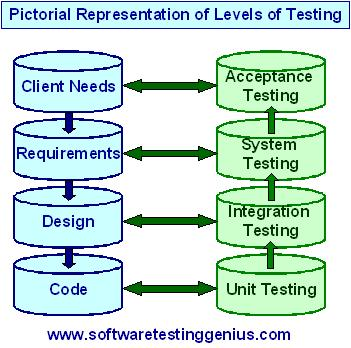
\includegraphics[width=.6\LW]{leveltest}
  \caption{Schéma testovacího modelu}
  \label{fig:router}
\end{figure}

\subsection{Testování programátorem (Developer testing)}
První a úplně nezbytnou částí testování by měl provádět programátoři. Programátor by si měl zkontrolovat jestli jde firmware přeložit a jestli jeho nová či opravená funkcionalita funguje správně. Dále by měl otestovat kód jiný programátor, který kód nepsal. To většinou provádí správce projektu při zařazování nové či upravené funkce do hlavní větve repozitáře. Všechny chyby odchycené v této fázi testování ušetří spoustu času stráveným v dalších fázích testování.

\subsection{Testování jednotek (Unit testing)}
Úroveň testování jednotek obsahuje testování jednotlvých jednotek software. Jako jednotku lze uvažovat objekt s jednou jedinou funkcionalitou například třídu, objekt, program či softwarový modul. Tato úroveň testování testuje správnost zdrojového kódu ne funkci celého programu. Velmi známým příkladem jsou JUnit testy v javě, kde ke každé třídě a metodě je psán i její test.

Tyto testy je výhodné použít při tvorbě nového projektu, jelikož s unit testy je potřeba počítat již při návrhu zdrojového kódu a při tomto návrhu zároveň tyto testy psát. Dopisování testů do již existujícího projektu by stálo velkou námahu a mnoho úprav kódu pro přizpůsobení programu pro unit testování.

Jelikož výrobky pro který je určen mnou navrhovaný testovací sytém jsou vyvýjeny již 10 let a dále přes devadesát procent firmwaru používá opensource řešení je nereálně přidat unit testování do testovacích procedur.


\subsection{Integrační testování (Integration testing)}


\subsection{SIT - Systémové testování (System testing)}


\subsection{UAT - Akceptační testování (Acceptance testing)}


\section{Testovací procesy}
\subsection{Manuální testování}
\subsection{Automatizované testování}
\subsection{Testování založené na modelech}


\section{Typy testování}

\subsection{Instalační testy}
\subsection{Testy splněním a selháním}
\subsection{Progresní a regresní testy}
\subsection{Smoke testy}
\subsection{Funkční a nefunkční testy}
\subsection{Testování bílé a černé skříňky}
\subsection{Statické a dynamické testy}

\section{Modely vývoje a testování}

\endinput
